\documentclass[conference]{IEEEtran}
\IEEEoverridecommandlockouts
% The preceding line is only needed to identify funding in the first footnote. If that is unneeded, please comment it out.
\usepackage{cite}
\usepackage{amsmath,amssymb,amsfonts}
\usepackage{algorithmic}
\usepackage[spanish]{babel} 
\usepackage[utf8]{inputenc}
\usepackage{graphicx}
\usepackage{textcomp}
\usepackage{hyperref}
\usepackage{multirow}
\usepackage{xcolor}
\usepackage{listings}
\usepackage{color}
\usepackage{multicol}
\usepackage{subcaption}
\usepackage[colorinlistoftodos]{todonotes}
\definecolor{mygreen}{rgb}{0,0.6,0}
\definecolor{mygray}{rgb}{0.5,0.5,0.5}
\definecolor{mymauve}{rgb}{0.58,0,0.82}
\def\BibTeX{{\rm B\kern-.05em{\sc i\kern-.025em b}\kern-.08em
    T\kern-.1667em\lower.7ex\hbox{E}\kern-.125emX}}
\lstset{
	belowcaptionskip=1\baselineskip,
	breaklines=true,
	xleftmargin=1.25cm,
	language=matlab,
	showstringspaces=false,
	basicstyle=\scriptsize \ttfamily,
	keywordstyle=\bfseries\color{green!40!black},
	commentstyle=\itshape\color{purple!40!black},
	identifierstyle=\color{blue},
	stringstyle=\color{orange},
	numbers=left,                    % where to put the line-numbers; possible values are (none, left, right)
	numbersep=15pt,
	numberstyle=\tiny\color{mygray}, % the style that is used for the line-numbers
	rulecolor=\color{black},
	columns =[l|l]flexible
}
\begin{document}

\title{
{\large \textsc{Escuela Superior Politécnica del Litoral}\\
Conmutación y Enrutamiento - TLMG1009: Proyecto Final
}\\
Sistemas de Respaldos Diarios Automáticos\\
}

\author{\IEEEauthorblockN{\textbf{Lino Ontano}}
\IEEEauthorblockA{	\textit{Telemática}
\\Guayaquil - Ecuador \\
lontano@espol.edu.ec
}
\and
\IEEEauthorblockN{\textbf{Julio Bodero}}
\IEEEauthorblockA{	\textit{Telemática}
\\Guayaquil - Ecuador \\
jcbodero@espol.edu.ec
}
\and
\IEEEauthorblockN{\textbf{Cesar Navas}}
\IEEEauthorblockA{	\textit{Telemática}
\\Guayaquil - Ecuador \\
cesanava@espol.edu.ec
}
\and
\IEEEauthorblockN{\textbf{Josue Martínez}}
\IEEEauthorblockA{	\textit{Telemática}
\\Guayaquil - Ecuador \\
josvmart@espol.edu.ec
}
\and
\IEEEauthorblockN{\textbf{Eduardo Veintimilla}}
\IEEEauthorblockA{	\textit{Telemática}
\\Guayaquil - Ecuador \\
edujvein@espol.edu.ec
}
}


\maketitle

\begin{abstract}
	Este proyecto permitirá explicar el funcionamiento del sistema de respaldos diarios automáticos, las herramientas utilizadas y las configuraciones pertinentes en los dispositivos intermediarios para poder realizar el respaldo y la consulta.
\end{abstract}

\section{Introducción}\label{sec:int}
Es necesario en una empresa, sea de grande o pequeña escala, tener las redes de sus sucursales siempre disponibles; de esta manera se garantiza el servicio que ofrece y el soporte a su empresa sin importar en que sucursal se encuentre el problema. Existen varias soluciones para mantener la alta disponibilidad de nuestra empresa, pero el riesgo de fallo siempre existirá y es ahí cuando el ingeniero de networking debe tener la solución disponible en un tiempo corto de respuesta. Por eso, la configuración de los dispositivos intermediarios de nuestra red es importante que esté al alcance de la persona encargada de dar soporte a la empresa, sin importar donde se encuentre. Este proyecto permite acceder a la configuración de los equipos intermediarios de nuestra red, en este caso utilizamos de ejemplo una red con tres dispositivos intermediarios, dos sucursales y una matriz. El aplicativo elaborado en el presente proyecto permite realizar un sistema de respaldo diario de estos dispositivos, así como una consulta de los mismos por fecha o por dispositivo. De esta manera ofrecemos una base de datos que servirá para ayudar a mitigar los problemas de fallas ya que se podrá acceder a los archivos de configuración de cualquier sucursal e identificar una posible mala configuración o un mal funcionamiento del mismo.
\begin{figure}[h]
	\centerline{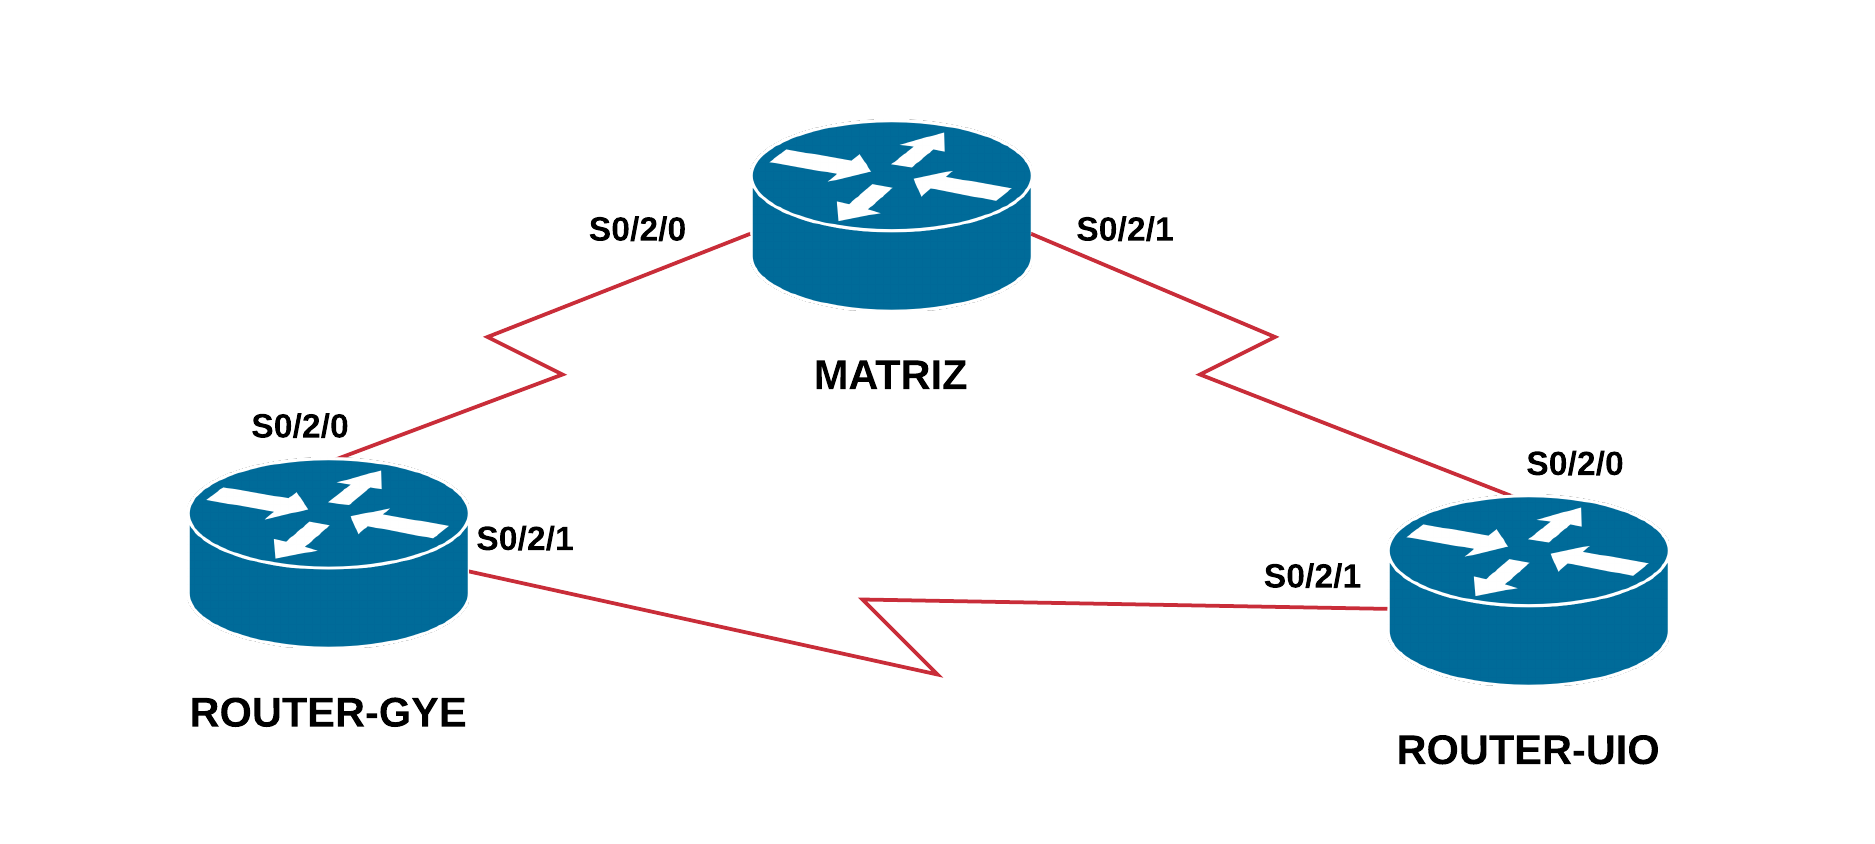
\includegraphics[width=0.51\textwidth]{img/int01.png}}
	\caption{\textit{Diagrama de red de las sucursales a respaldar}}
	\label{fig:ant00}
\end{figure}
\section{Antecedentes}\label{sec:ant}
\subsection{\textbf{ Dispositivos intermediarios:}}
Los dispositivos intermediarios interconectan dispositivos finales. Estos dispositivos proporcionan conectividad y operan detrás de escena para asegurar que los datos fluyan a través de la red. Los dispositivos intermediarios conectan los hosts individuales a la red y pueden conectar varias redes individuales para formar una internetwork.\\
Los siguientes son ejemplos de dispositivos de red intermediarios:
\begin{itemize}
\item Acceso a la red (switches y puntos de acceso inalámbrico)
\item Internetworking (routers)
\item Seguridad (firewalls)
\end{itemize}

\subsection{\textbf{Protocolo SSH:}}
\begin{figure}[h]
	\centerline{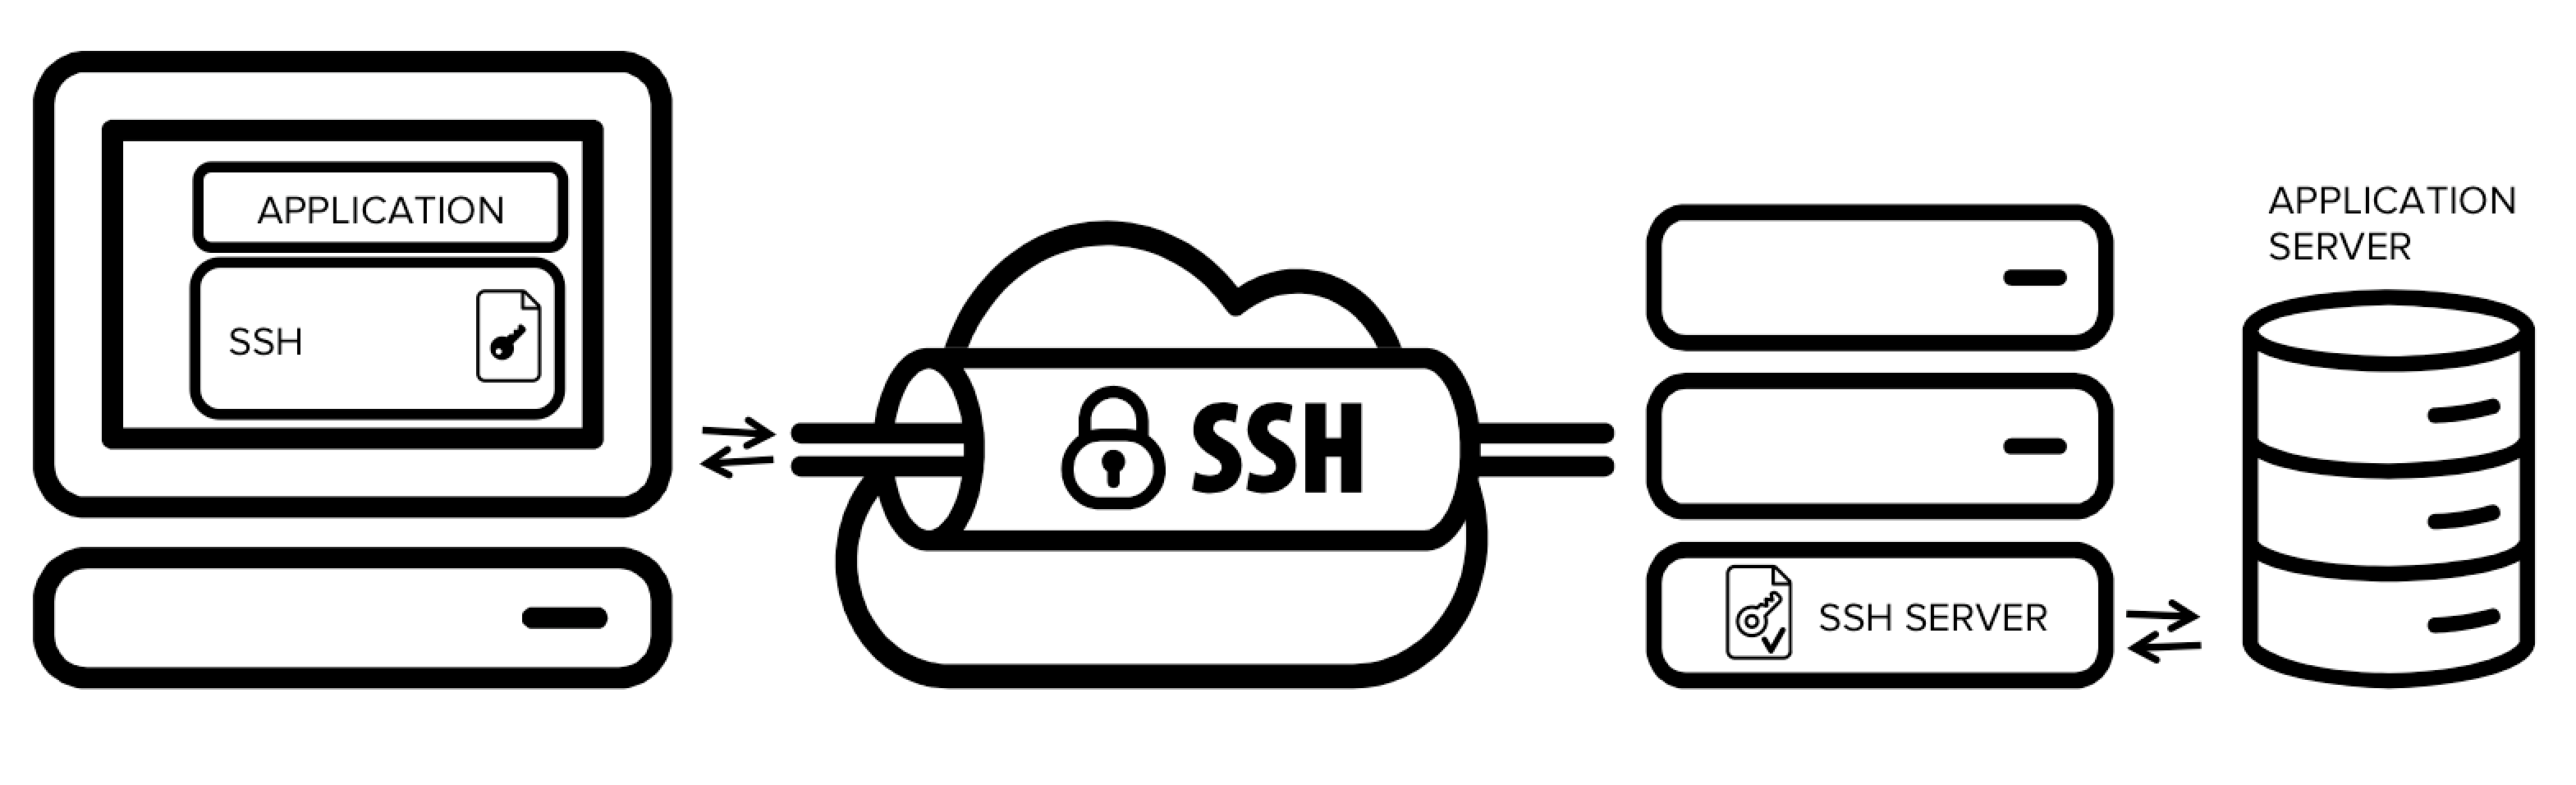
\includegraphics[width=0.45\textwidth]{img/ant02.png}}
	\caption{\textit{Funcionamiento del protocolo SSH}}
	\label{fig:ant02}
\end{figure}

SSH (o \textit{Secure SHell}) es el nombre de un protocolo y del programa que lo implementa cuya principal función es el acceso remoto a un servidor por medio de un canal seguro en el que toda la información está cifrada. SSH trabaja de forma similar a como se hace con \textit{telnet}. La diferencia principal es que SSH usa técnicas de cifrado que hacen que la información que viaja por el medio de comunicación vaya de manera no legible, evitando que terceras personas puedan descubrir el usuario y contraseña de la conexión ni lo que se escribe durante toda la sesión; aunque es posible atacar este tipo de sistemas por medio de ataques de REPLAY y manipular así la información entre destinos. El protocolo TCP asignado es el 22.

\subsection{\textbf{ Protocolo de Transferencia de Archivos FTP:}}
FTP es un protocolo de red para la transferencia de archivos entre sistemas conectados a una red TCP (Transmission Control Protocol), basado en la arquitectura cliente-servidor. Desde un equipo cliente se puede conectar a un servidor para descargar archivos desde él o para enviarle archivos, independientemente del sistema operativo utilizado en cada equipo.\\
El servicio FTP es ofrecido por la capa de aplicación del modelo de capas de red TCP/IP al usuario, utilizando normalmente el puerto de red 20 y el 21. Un problema básico de FTP es que está pensado para ofrecer la máxima velocidad en la conexión, pero no la máxima seguridad, ya que todo el intercambio de información, desde el login y password del usuario en el servidor hasta la transferencia de cualquier archivo, se realiza en texto plano sin ningún tipo de cifrado, con lo que un posible atacante puede capturar este tráfico, acceder al servidor y/o apropiarse de los archivos transferidos.

\textit{Asterisk} incluye muchas características que anteriormente sólo estaban disponibles en costosos sistemas propietarios PBX, como buzón de voz, conferencias, IVR, distribución automática de llamadas, y otras muchas. Los usuarios pueden crear nuevas funcionalidades escribiendo un dialplan en el lenguaje de script de \textit{Asterisk} o añadiendo módulos escritos en lenguaje C o en cualquier otro lenguaje de programación soportado en GNU/Linux.\\
Uno de los puntos fuertes del software \textit{Asterisk} es que permite la unificación de tecnologías: VoIP, GSM y PSTN.\\
\textit{Asterisk} se empieza a adoptar en algunos entornos corporativos como una gran solución de bajo coste junto con SER (Sip Express Router).


\subsection{\textbf{ OSPF:}}
\textit{Open Shortest Path First} (OSPF), Primer Camino Más Corto, es un protocolo de red para encaminamiento jerárquico de pasarela interior o Interior Gateway Protocol (IGP), que usa el algoritmo Dijkstra, para calcular la ruta más corta entre dos nodos.\\
Su medida de métrica se denomina cost, y tiene en cuenta diversos parámetros tales como el ancho de banda y la congestión de los enlaces. OSPF construye además una base de datos enlace-estado (Link-State Database, LSDB) idéntica en todos los routers de la zona.\\
Una red OSPF se puede descomponer en regiones (áreas) más pequeñas. Hay un área especial llamada área backbone que forma la parte central de la red a la que se encuentran conectadas el resto de áreas de la misma. Las rutas entre las diferentes áreas circulan siempre por el backbone, por lo tanto todas las áreas deben conectar con el backbone. Si no es posible hacer una conexión directa con el backbone, se puede hacer un enlace virtual entre redes.

\section{Desarrollo del concepto}\label{sec:ddc}
\begin{figure}[h]
	\centerline{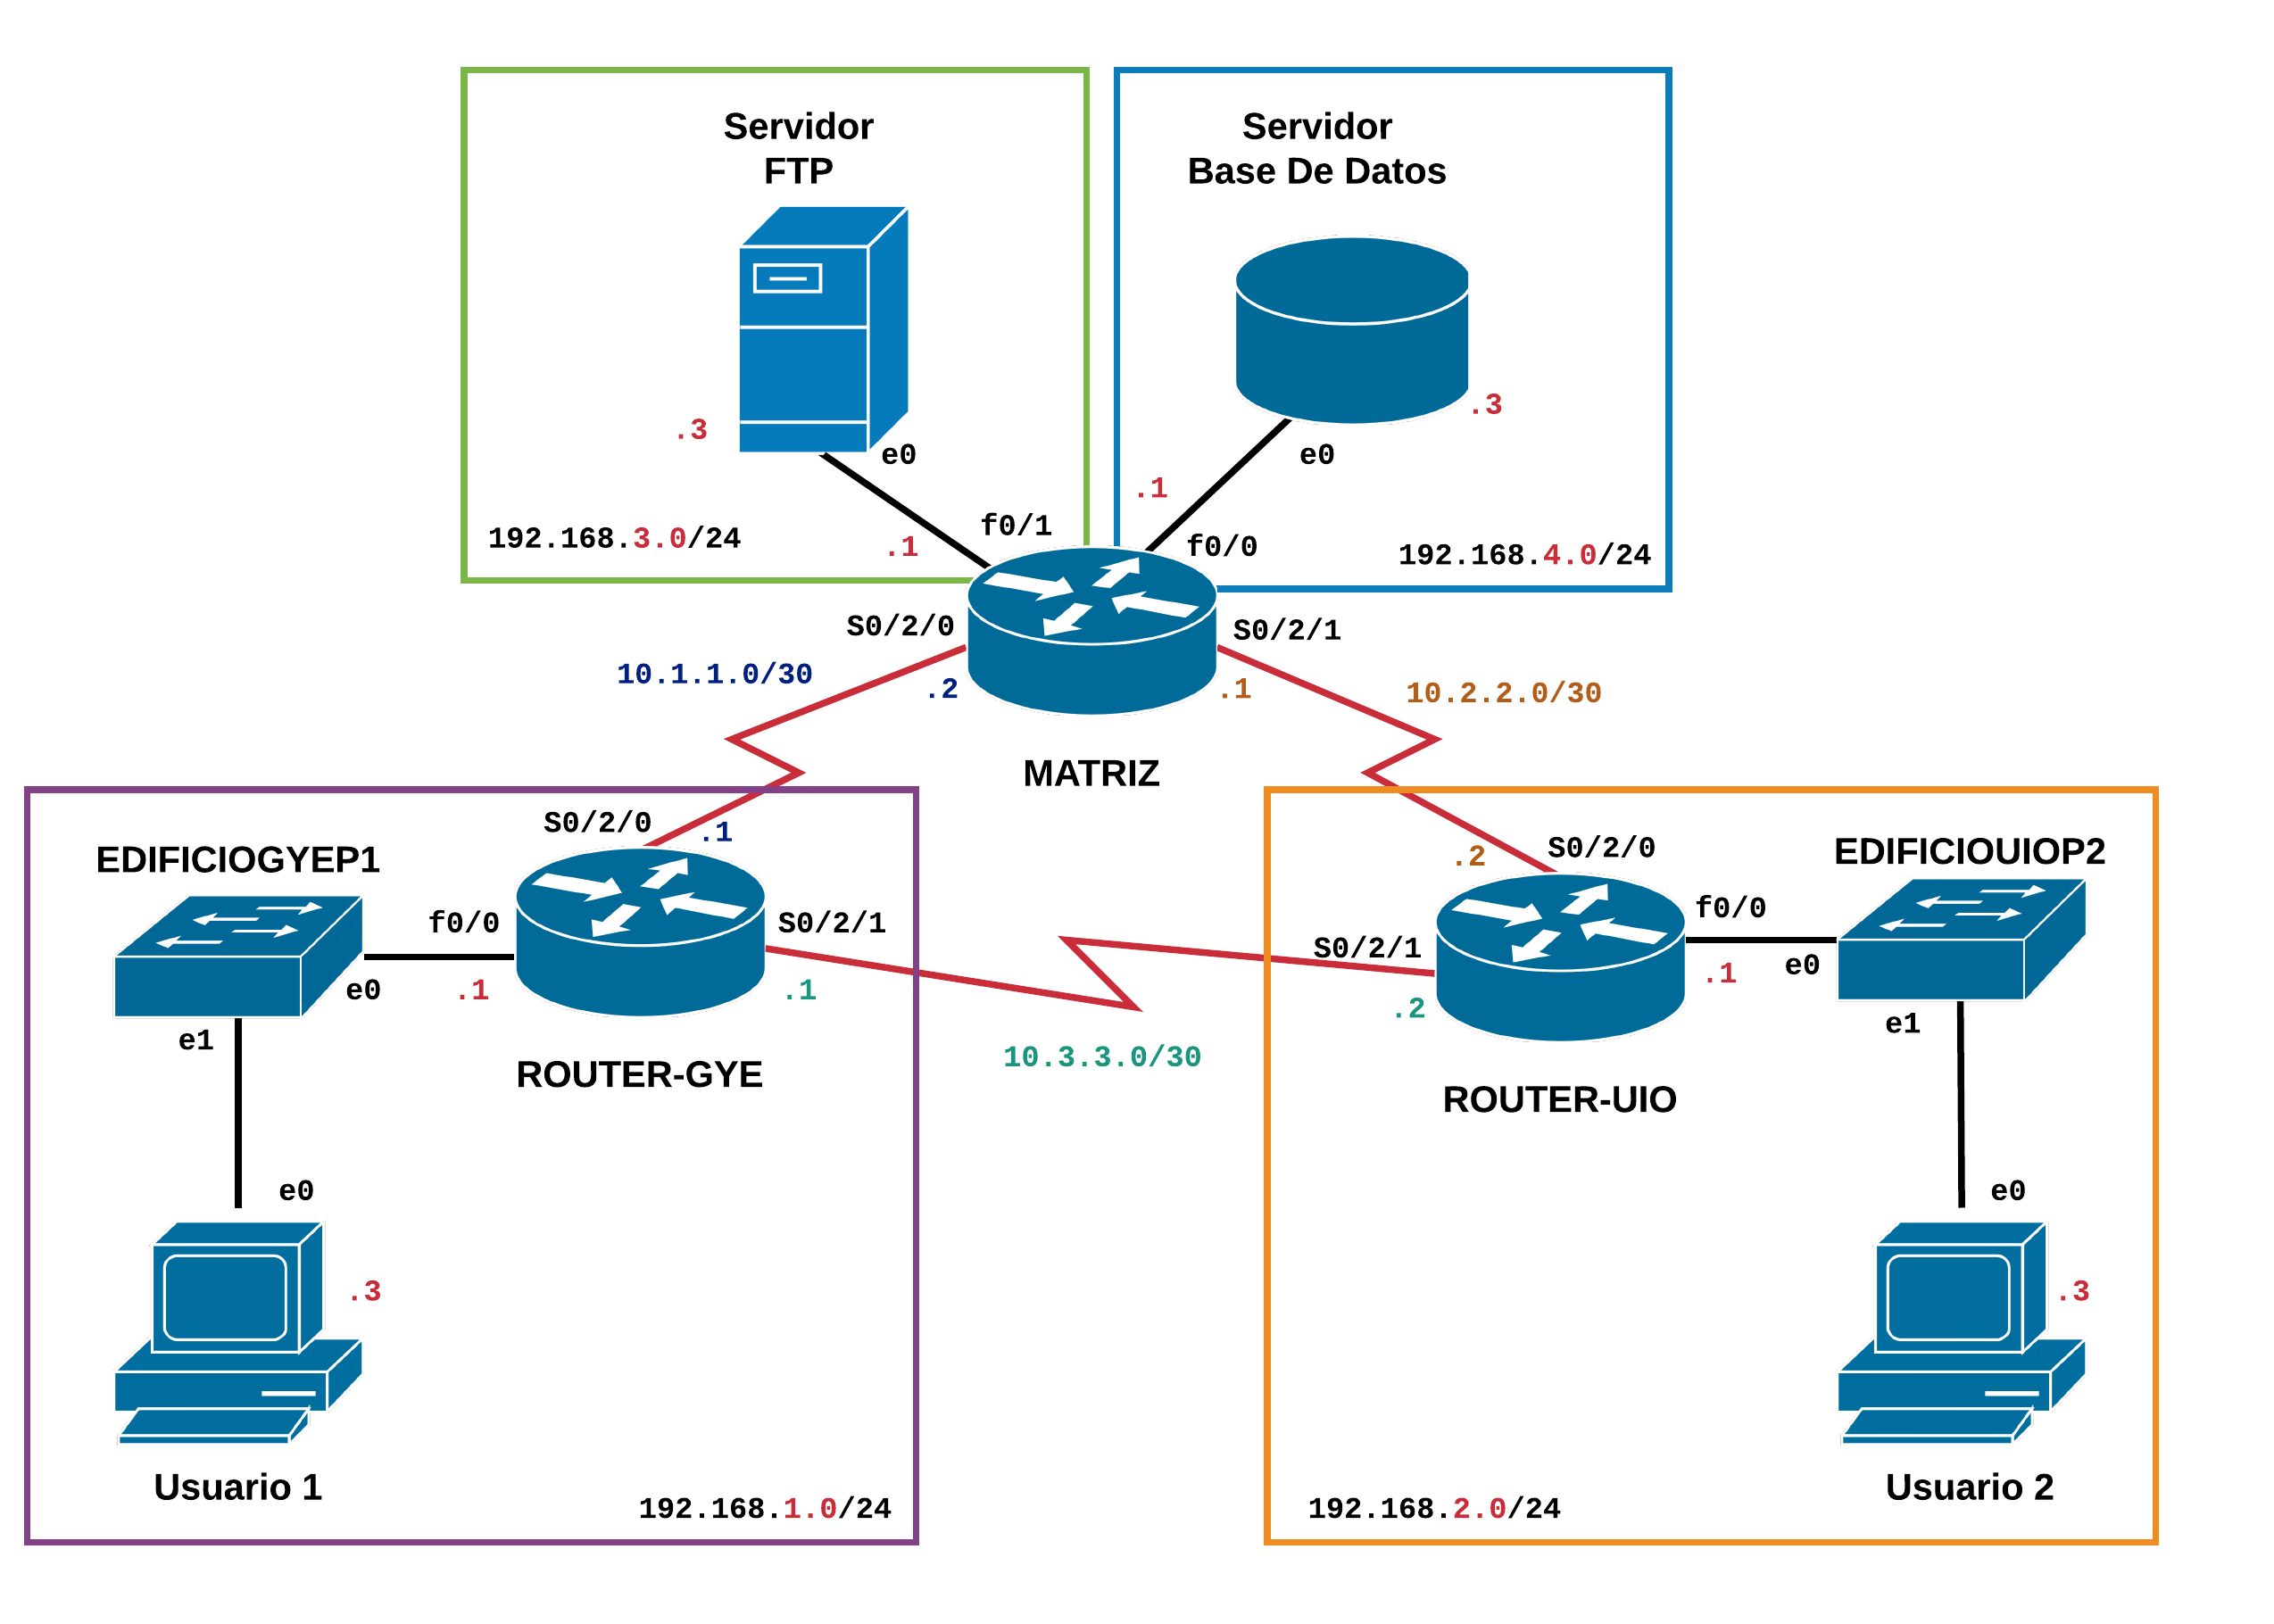
\includegraphics[width=0.50\textwidth]{img/desa01.png}}
	\caption{\textit{Diagrama completo de red de nuestra empresa. Se observa que los dispositivos intermediarios interconectan dos sucursales diferentes con la matriz.}}
	\label{fig:ddc01}
\end{figure}

Para el desarrollo de nuestro proyecto, nos basamos en la red de la figura \ref{fig:ddc01}, donde planteamos que desde cualquier red de las sucursales, por medio de un aplicativo, poder consultar a cualquier dispositivo intermediario presente de la red y hacer respaldos y consultas de los mismos. Para ello, el aplicativo cuenta con autenticación para ser utilizado, es decir la empresa tendrá una base de datos de usuarios que pueden realizar la gestión de resplado y consultas por medio del aplicativo, además de descargar dichos archivos de consultas. Todo estas conexiones se realizan por medio del protocolo SSH, que nos permite hacer conexión y adquirir los datos de los dispositivos intermediarios de manera segura.

\section{Diseño e Implementación}
El desarrollo del presente proyecto se realizó basándonos en el diagrama de la figura \ref{fig:ddc01}, teniendo que configurar cada dispositivo presente en el diagrama de acuerdo a las redes en las que se encuentran. Nos basamos en la tabla \ref{tab:dir01} para asignar las direcciones IPs de los dispositivos finales y de las interfaces de los dispositivos intermediarios. \\
\begin{table}[h]
\begin{center}
	\begin{tabular}{|l|l|l|c|}
	\hline
	\textbf{Dispositivo} &\textbf{Interfaz} &\textbf{Dirección/Máscara} &\textbf{ Gateway }\\ \hline
	\multirow{3}{*}{ROUTER-GYE}& f0/0 & 192.168.1.1/24 & n/a\\ \cline{2-4}
	&s0/2/0  &10.1.1.1/30 & n/a \\ \cline{2-4}
	&s0/2/1 &10.3.3.1/30 & n/a\\ \hline
	\multirow{3}{*}{ROUTER-UIO}& f0/0 & 192.168.2.1/24 & n/a\\ \cline{2-4}
	&s0/2/0  &10.2.2.2/30 & n/a \\ \cline{2-4}
	&s0/2/1 &10.3.3.2/30 & n/a\\ \hline
	\multirow{3}{*}{MATRIZ}& f0/0 & 192.168.3.1/24 & n/a\\ \cline{2-4}
	& f0/1 & 192.168.4.1/24 & n/a\\ \cline{2-4}
	&s0/2/0  &10.1.1.2/30 & n/a \\ \cline{2-4}
	&s0/2/1 &10.2.2.1/30 & n/a\\ \hline
	Usuario 1 & NIC & 192.168.1.3/24 &192.168.1.1 \\\hline
	Usuario 2 & NIC & 192.168.2.3/24 &192.168.2.1 \\\hline
	Servidor DB & NIC & 192.168.3.3/24 &192.168.3.1 \\\hline
	Servidor FTP & NIC & 192.168.4.3/24 &192.168.4.1 \\\hline
\end{tabular}\vspace{0.25cm}
\caption{\textit{Direccionamiento de red de la figura \ref{fig:ddc01}}}
\label{tab:dir01}
\end{center}
\end{table}\\
Observe que las interfaces de los dispositivos intermediarios son importantes en este proceso, ya que una interfaz mal configurada hará que no exista conectividad entre redes. Para interconectar las redes utilizamos el protocolo OSPF, el cual se configura en cada enrutador sucursal y en el enrutador matriz.\\
La configuración de cada enrutador dependerá del cuadro de direcciones \ref{tab:dir01}, se le asigna en primer lugar el direccionamiento y se habilita el protocolo OSPF para interconectar las redes. Para el caso del enrutador MATRIZ, sería como sigue:\\

\lstinputlisting{/home/lianontano/Documentos/LaTeX/CE-Proyecto/2T2018_PROYECTO_SistemaDeRespaldosDiariosAutomaticos_GRUPO1/archivosConfiguracion/conf-MATRIZ.txt}

Ahora, ya teniendo la red configurada, se requiere el acceso a los enrutadores vía SSH, para lo que de igual manera requiere ser configurado para cada enrutador, como sigue:

\lstinputlisting{/home/lianontano/Documentos/LaTeX/CE-Proyecto/2T2018_PROYECTO_SistemaDeRespaldosDiariosAutomaticos_GRUPO1/archivosConfiguracion/SSh-ROUTER-MATRIZ.txt}

Ya en este punto, podemos acceder a los enrutadores vía SSH.\\
La parte de la aplicación, requiere un servidor FTP y un servidor de Base de Datos; ambos en este caso, se encuentran conectados en el enrutador MATRIZ. El servidor FTP permitirá la descarga de los archivos que se generen de los respaldos y el servidor de la base de datos llevará un control de las actividades que se realicen por medio de la aplicación.\\
La aplicación fue desarrollada en Java, y es ella la que realiza la conexión por SSH con los enrutadores y genera los archivos de configuración de cada enrutador. El administrador selecciona cual enrutador desea generar respaldo o consultar los respaldos generados como se observa en la figura \ref{fig:ap01}.\\
Para mayor información acerca de la aplicación pueden consultar el repositorio de gitHub de este proyecto \href{https://github.com/jcbodero/2T2018_PROYECTO_SistemaDeRespaldosDiariosAutomaticos_GRUPO1}{\textcolor{red}{\textbf{aquí}}}.
\begin{figure}[h]
    \begin{subfigure}[h]{0.5\textwidth}
       \centerline{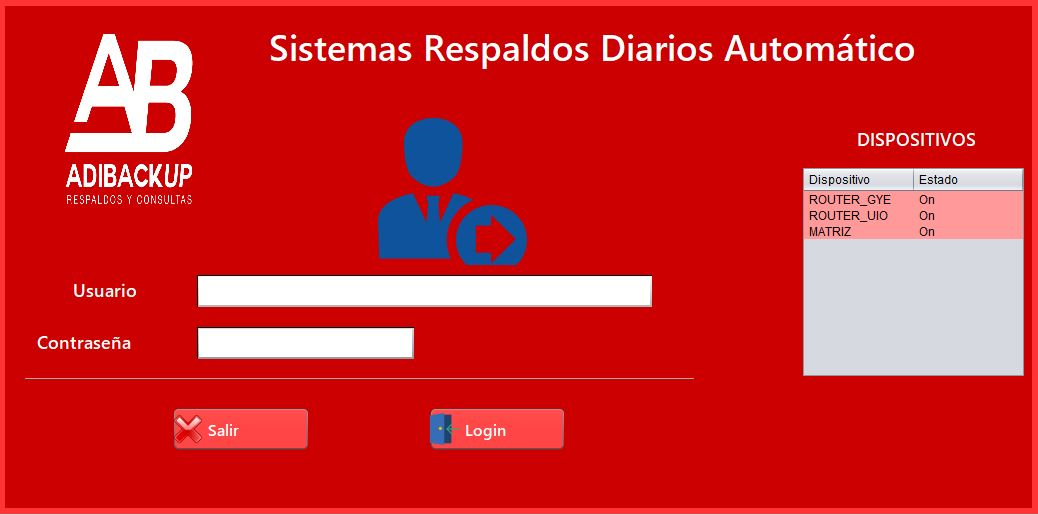
\includegraphics[width=0.7\textwidth]{img/ap01.jpg}}
        \caption{Inicio de sesión}

    \end{subfigure}
    ~ %add desired spacing between images, e. g. ~, \quad, \qquad, \hfill etc.
     \begin{subfigure}[h]{0.5\textwidth}
        \centerline{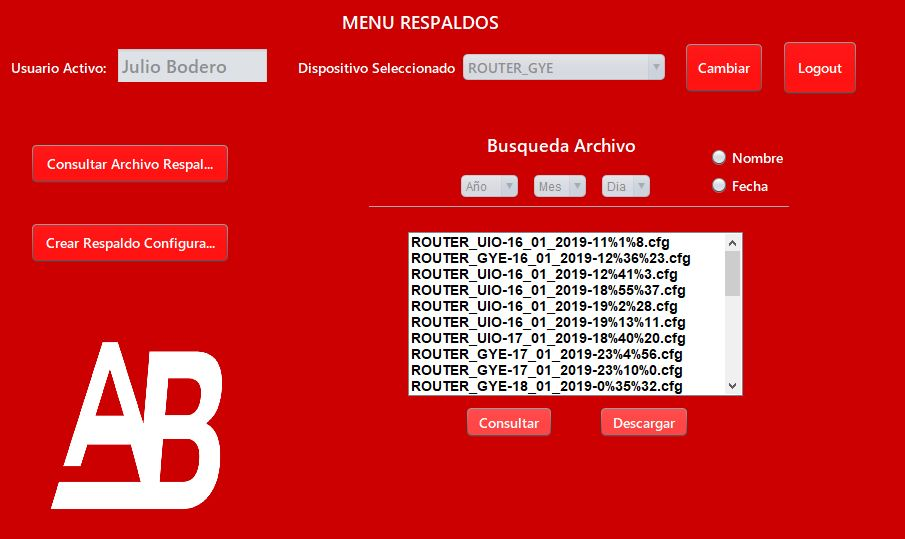
\includegraphics[width=0.7\textwidth]{img/ap02.jpg}}
        \caption{Consulta de archivos de respaldo}

    \end{subfigure}
    \caption{\textit{Interfaz gráfica de la aplicación.}}
\label{fig:ap01}
\end{figure}


\section{Conclusiones}
\begin{itemize}
	\item Es importante el manejo de logs en redes que demanda el uso de varios dispositivos ya que ayuda a detectar fallas y corregir errores en los dispositivos causantes.
	\item La configuración de los dispositivos es el punto clave para que exista forma de conectar la aplicación con nuestra red.
	\item El sistema de respaldo diarios permite control remoto de dispositivos de una empresa ayudando al soporte técnico a reducir gastos.
\end{itemize}
\section{Recomendaciones}
\begin{itemize}
	\item El protocolo FTP a largo plazo se tendrá que cambiar por un protocolo más seguro.
	\item Es indispensable realizar una aplicación compatible con dispositivos móviles para hacer que el sistema sea multiplataforma, de esta manera dará mayor alcance el presente proyecto.
\end{itemize}

\begin{thebibliography}{00}
\bibitem{b1}  J. Moy: RFC 2328, ``OSPF Version 2'' , IETF (abril de 1998)
\bibitem{b2} Daniel J. Barrett, Richard E. Silverman, and Robert G. Byrnes, ``SSH: The Secure Shell (The Definitive Guide)", O'Reilly 2005 (2nd edition). ISBN 0-596-00895-3.
\bibitem{b3} Gleason, Mike, ``The File Transfer Protocol and Your Firewall/NAT'',  Ncftp.com (2005).

\end{thebibliography}

\end{document}
